\documentclass{standalone}
\usepackage{tikz}
\usetikzlibrary{patterns, positioning}
\usepackage[sfdefault]{ClearSans} %% option 'sfdefault' activates Clear Sans as the default text font
\usepackage[T1]{fontenc}

\begin{document}
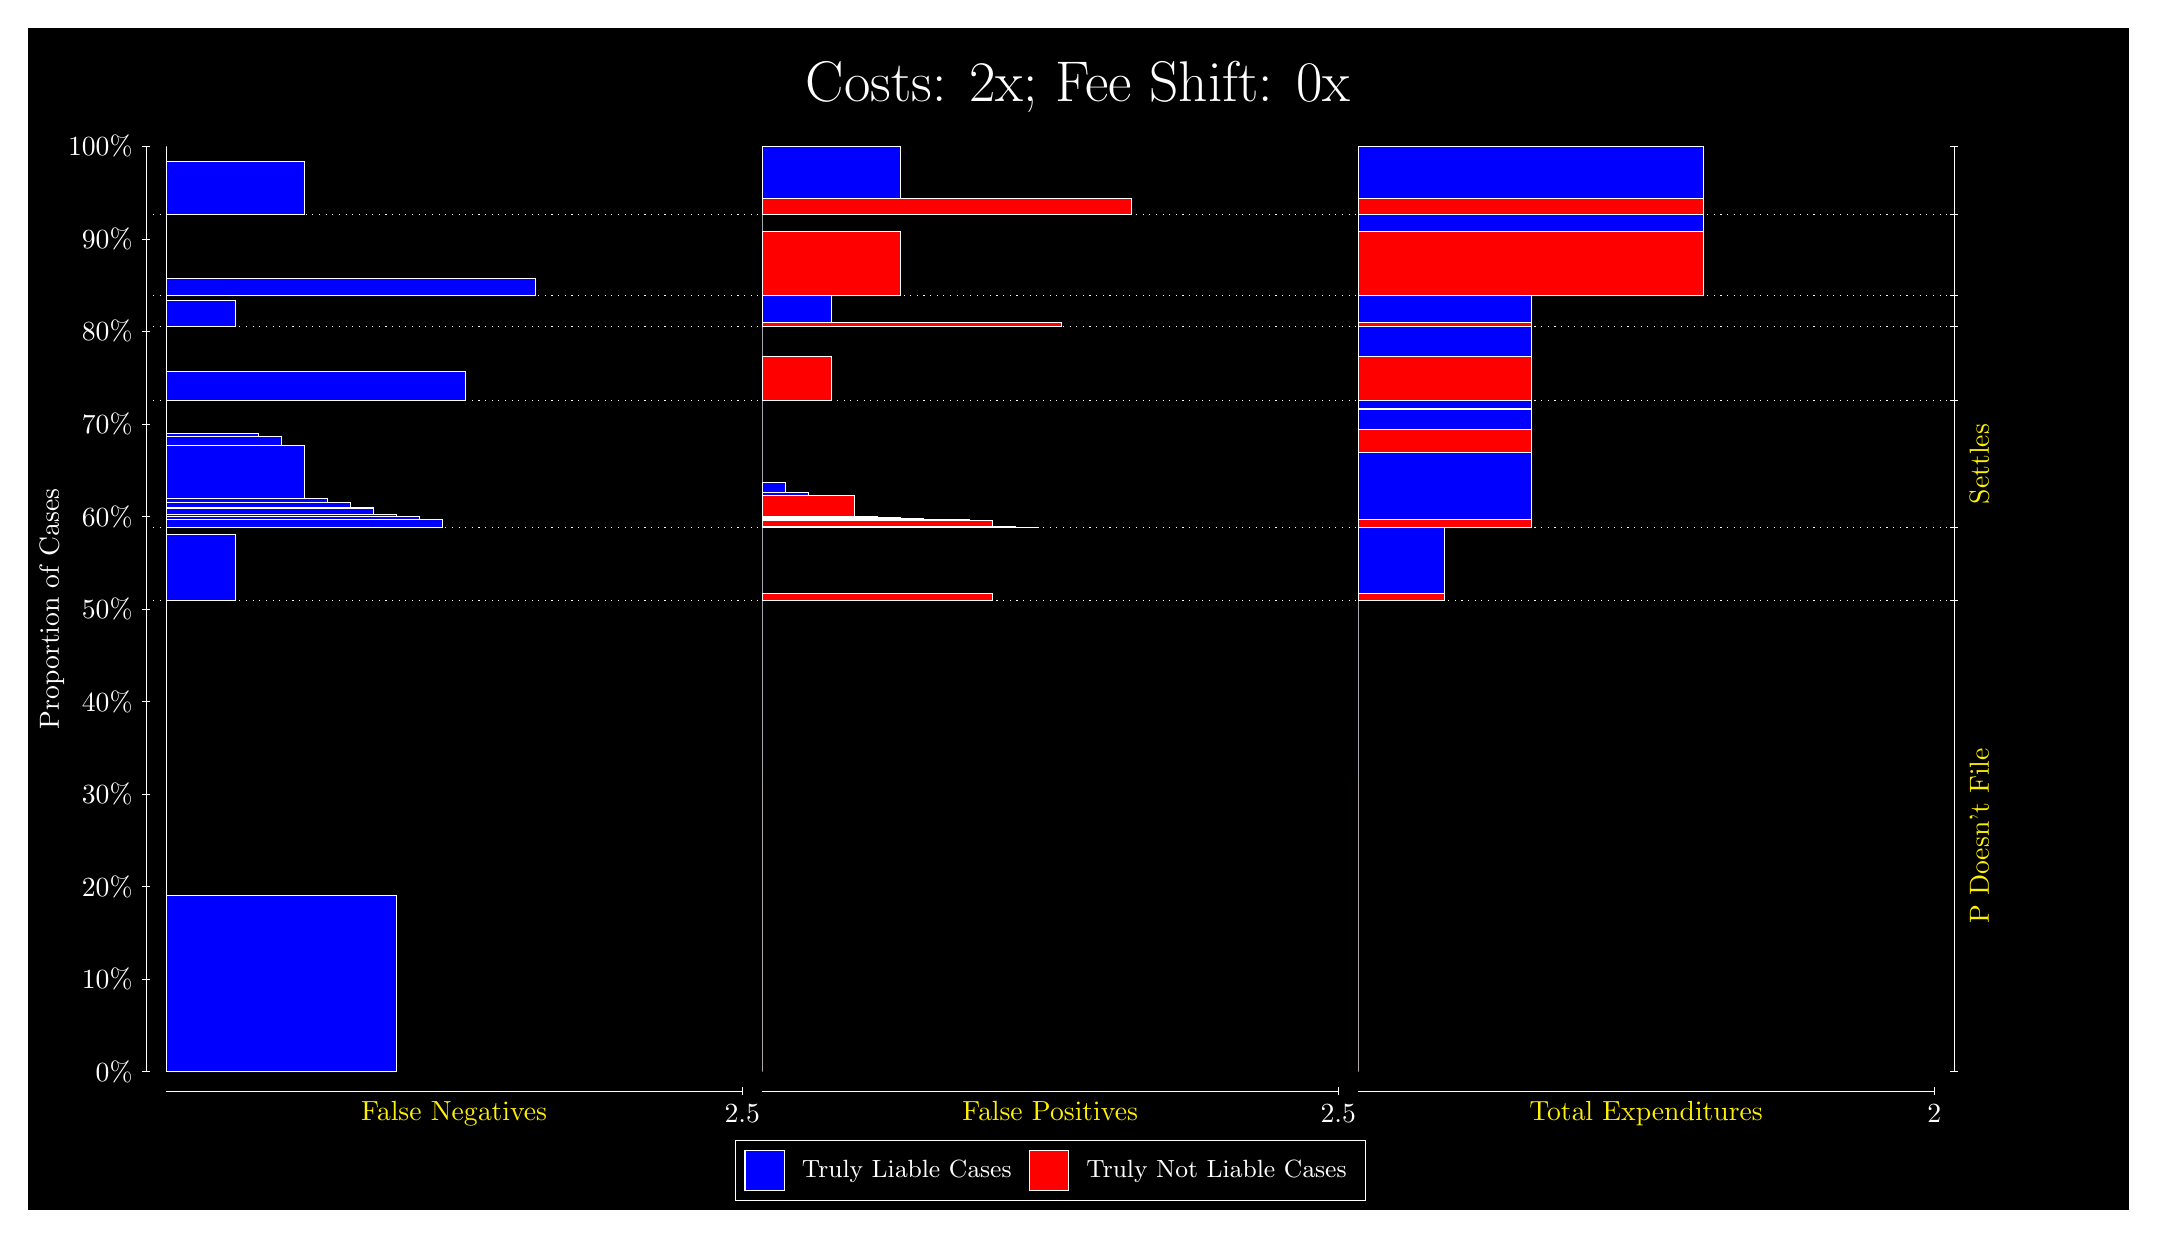
\begin{tikzpicture}
\draw[fill=black] (0,0) rectangle (26.667,15);
\draw[text=white] (0,13.5) rectangle (26.667,15) node[midway] {\huge Costs: 2x; Fee Shift: 0x};
\draw[white, very thin] (1.5,1.75) -- (1.5,13.5);
\node[rotate=90, text=white, anchor=center] at (0.3, 7.625) {Proportion of Cases};
\draw[white, very thin] (1.45,1.75) -- (1.55,1.75);
\node[text=white, anchor=east] at (1.45, 1.75) {0\%};
\draw[white, very thin] (1.45,2.925) -- (1.55,2.925);
\node[text=white, anchor=east] at (1.45, 2.925) {10\%};
\draw[white, very thin] (1.45,4.1) -- (1.55,4.1);
\node[text=white, anchor=east] at (1.45, 4.1) {20\%};
\draw[white, very thin] (1.45,5.275) -- (1.55,5.275);
\node[text=white, anchor=east] at (1.45, 5.275) {30\%};
\draw[white, very thin] (1.45,6.45) -- (1.55,6.45);
\node[text=white, anchor=east] at (1.45, 6.45) {40\%};
\draw[white, very thin] (1.45,7.625) -- (1.55,7.625);
\node[text=white, anchor=east] at (1.45, 7.625) {50\%};
\draw[white, very thin] (1.45,8.8) -- (1.55,8.8);
\node[text=white, anchor=east] at (1.45, 8.8) {60\%};
\draw[white, very thin] (1.45,9.975) -- (1.55,9.975);
\node[text=white, anchor=east] at (1.45, 9.975) {70\%};
\draw[white, very thin] (1.45,11.15) -- (1.55,11.15);
\node[text=white, anchor=east] at (1.45, 11.15) {80\%};
\draw[white, very thin] (1.45,12.325) -- (1.55,12.325);
\node[text=white, anchor=east] at (1.45, 12.325) {90\%};
\draw[white, very thin] (1.45,13.5) -- (1.55,13.5);
\node[text=white, anchor=east] at (1.45, 13.5) {100\%};

\draw[white, very thin] (24.457,1.75) -- (24.457,13.5);
\draw[white, very thin] (24.407,1.75) -- (24.507,1.75);
\node[anchor=west] at (24.407, 1.75) {};
\draw[white, very thin] (24.407,7.7333) -- (24.507,7.7333);
\node[anchor=west] at (24.407, 7.7333) {};
\draw[white, very thin] (24.407,8.6601) -- (24.507,8.6601);
\node[anchor=west] at (24.407, 8.6601) {};
\draw[white, very thin] (24.407,10.269) -- (24.507,10.269);
\node[anchor=west] at (24.407, 10.269) {};
\draw[white, very thin] (24.407,11.216) -- (24.507,11.216);
\node[anchor=west] at (24.407, 11.216) {};
\draw[white, very thin] (24.407,11.602) -- (24.507,11.602);
\node[anchor=west] at (24.407, 11.602) {};
\draw[white, very thin] (24.407,12.639) -- (24.507,12.639);
\node[anchor=west] at (24.407, 12.639) {};
\draw[white, very thin] (24.407,13.5) -- (24.507,13.5);
\node[anchor=west] at (24.407, 13.5) {};

\draw[white, very thin, fill=blue] (1.75,1.75) rectangle (4.6775,3.9927);
\draw[white, very thin, fill=red] (1.75,3.9927) rectangle (1.75,7.7333);
\draw[white, very thin, fill=blue] (1.75,7.7333) rectangle (2.6283,8.5691);
\draw[white, very thin, fill=red] (1.75,8.5691) rectangle (1.75,8.6601);
\draw[white, very thin, fill=blue] (1.75,8.6601) rectangle (5.2631,8.7673);
\draw[white, very thin, fill=blue] (1.75,8.7673) rectangle (4.9703,8.7964);
\draw[white, very thin, fill=blue] (1.75,8.7964) rectangle (4.6775,8.8291);
\draw[white, very thin, fill=blue] (1.75,8.8291) rectangle (4.3848,8.9088);
\draw[white, very thin, fill=blue] (1.75,8.9088) rectangle (4.3848,8.9182);
\draw[white, very thin, fill=blue] (1.75,8.9182) rectangle (4.092,8.984);
\draw[white, very thin, fill=blue] (1.75,8.984) rectangle (3.7993,9.0347);
\draw[white, very thin, fill=blue] (1.75,9.0347) rectangle (3.5065,9.7018);
\draw[white, very thin, fill=blue] (1.75,9.7018) rectangle (3.2138,9.8218);
\draw[white, very thin, fill=blue] (1.75,9.8218) rectangle (2.921,9.8606);
\draw[white, very thin, fill=red] (1.75,9.8606) rectangle (1.75,10.269);
\draw[white, very thin, fill=blue] (1.75,10.269) rectangle (5.5558,10.648);
\draw[white, very thin, fill=red] (1.75,10.648) rectangle (1.75,11.216);
\draw[white, very thin, fill=blue] (1.75,11.216) rectangle (2.6283,11.55);
\draw[white, very thin, fill=red] (1.75,11.55) rectangle (1.75,11.602);
\draw[white, very thin, fill=blue] (1.75,11.602) rectangle (6.4341,11.82);
\draw[white, very thin, fill=red] (1.75,11.82) rectangle (1.75,12.639);
\draw[white, very thin, fill=blue] (1.75,12.639) rectangle (3.5065,13.305);
\draw[white, very thin, fill=red] (1.75,13.305) rectangle (1.75,13.5);
\draw[white, very thin, fill=red] (9.3189,1.75) rectangle (9.3189,5.4905);
\draw[white, very thin, fill=blue] (9.3189,5.4905) rectangle (9.3189,7.7333);
\draw[white, very thin, fill=red] (9.3189,7.7333) rectangle (12.246,7.8243);
\draw[white, very thin, fill=blue] (9.3189,7.8243) rectangle (9.3189,8.6601);
\draw[white, very thin, fill=red] (9.3189,8.6601) rectangle (12.832,8.6647);
\draw[white, very thin, fill=red] (9.3189,8.6647) rectangle (12.539,8.6794);
\draw[white, very thin, fill=red] (9.3189,8.6794) rectangle (12.246,8.7535);
\draw[white, very thin, fill=red] (9.3189,8.7535) rectangle (11.954,8.7601);
\draw[white, very thin, fill=red] (9.3189,8.7601) rectangle (11.661,8.769);
\draw[white, very thin, fill=red] (9.3189,8.769) rectangle (11.368,8.7811);
\draw[white, very thin, fill=red] (9.3189,8.7811) rectangle (11.075,8.7901);
\draw[white, very thin, fill=red] (9.3189,8.7901) rectangle (10.783,8.8034);
\draw[white, very thin, fill=red] (9.3189,8.8034) rectangle (10.49,9.0686);
\draw[white, very thin, fill=blue] (9.3189,9.0686) rectangle (9.9044,9.1074);
\draw[white, very thin, fill=blue] (9.3189,9.1074) rectangle (9.6116,9.2274);
\draw[white, very thin, fill=blue] (9.3189,9.2274) rectangle (9.3189,10.269);
\draw[white, very thin, fill=red] (9.3189,10.269) rectangle (10.197,10.838);
\draw[white, very thin, fill=blue] (9.3189,10.838) rectangle (9.3189,11.216);
\draw[white, very thin, fill=red] (9.3189,11.216) rectangle (13.125,11.268);
\draw[white, very thin, fill=blue] (9.3189,11.268) rectangle (10.197,11.602);
\draw[white, very thin, fill=red] (9.3189,11.602) rectangle (11.075,12.422);
\draw[white, very thin, fill=blue] (9.3189,12.422) rectangle (9.3189,12.639);
\draw[white, very thin, fill=red] (9.3189,12.639) rectangle (14.003,12.834);
\draw[white, very thin, fill=blue] (9.3189,12.834) rectangle (11.075,13.5);
\draw[white, very thin, fill=red] (16.888,1.75) rectangle (16.888,5.4905);
\draw[white, very thin, fill=blue] (16.888,5.4905) rectangle (16.888,7.7333);
\draw[white, very thin, fill=red] (16.888,7.7333) rectangle (17.986,7.8243);
\draw[white, very thin, fill=blue] (16.888,7.8243) rectangle (17.986,8.6601);
\draw[white, very thin, fill=red] (16.888,8.6601) rectangle (19.083,8.7578);
\draw[white, very thin, fill=blue] (16.888,8.7578) rectangle (19.083,9.6109);
\draw[white, very thin, fill=red] (16.888,9.6109) rectangle (19.083,9.9091);
\draw[white, very thin, fill=blue] (16.888,9.9091) rectangle (19.083,10.158);
\draw[white, very thin, fill=red] (16.888,10.158) rectangle (19.083,10.17);
\draw[white, very thin, fill=blue] (16.888,10.17) rectangle (19.083,10.269);
\draw[white, very thin, fill=red] (16.888,10.269) rectangle (19.083,10.838);
\draw[white, very thin, fill=blue] (16.888,10.838) rectangle (19.083,11.216);
\draw[white, very thin, fill=red] (16.888,11.216) rectangle (19.083,11.268);
\draw[white, very thin, fill=blue] (16.888,11.268) rectangle (19.083,11.602);
\draw[white, very thin, fill=red] (16.888,11.602) rectangle (21.279,12.422);
\draw[white, very thin, fill=blue] (16.888,12.422) rectangle (21.279,12.639);
\draw[white, very thin, fill=red] (16.888,12.639) rectangle (21.279,12.834);
\draw[white, very thin, fill=blue] (16.888,12.834) rectangle (21.279,13.5);
\draw[white, dotted] (1.5,7.7333) -- (24.457,7.7333);
\draw[white, dotted] (1.5,8.6601) -- (24.457,8.6601);
\draw[white, dotted] (1.5,10.269) -- (24.457,10.269);
\draw[white, dotted] (1.5,11.216) -- (24.457,11.216);
\draw[white, dotted] (1.5,11.602) -- (24.457,11.602);
\draw[white, dotted] (1.5,12.639) -- (24.457,12.639);
\draw[white, very thin] (1.75,1.5) -- (9.0689,1.5);
\node[text=yellow, anchor=north] at (5.4094, 1.5) {False Negatives};
\draw[white, very thin] (9.0689,1.45) -- (9.0689,1.55);
\node[text=white, anchor=north] at (9.0689, 1.45) {2.5};

\draw[white, very thin] (9.3189,1.5) -- (16.638,1.5);
\node[text=yellow, anchor=north] at (12.978, 1.5) {False Positives};
\draw[white, very thin] (16.638,1.45) -- (16.638,1.55);
\node[text=white, anchor=north] at (16.638, 1.45) {2.5};

\draw[white, very thin] (16.888,1.5) -- (24.207,1.5);
\node[text=yellow, anchor=north] at (20.547, 1.5) {Total Expenditures};
\draw[white, very thin] (24.207,1.45) -- (24.207,1.55);
\node[text=white, anchor=north] at (24.207, 1.45) {2};

\node[text=yellow, centered, rotate=90] at (24.777, 4.7416) {P Doesn't File};

\node[text=yellow, centered, rotate=90] at (24.777, 9.4646) {Settles};





\draw (12.978300999999998,1.5) node[draw=none] (baseCoordinate) {};
\begin{scope}[align=center]
        \matrix[scale=0.5, draw=white, below=0.5cm of baseCoordinate, nodes={draw}, column sep=0.1cm]{
            \node[rectangle, draw, minimum width=0.5cm, minimum height=0.5cm, fill=blue] {}; &
            \node[draw=none, font=\small, text=white] (B) {Truly Liable Cases}; &
            \node[rectangle, draw, minimum width=0.5cm, minimum height=0.5cm, fill=red] {}; &
            \node[draw=none, font=\small, text=white] (B) {Truly Not Liable Cases}; \\
            };
\end{scope}

\end{tikzpicture}
\end{document}